
\documentclass{beamer}
%\beamertemplateshadingbackground{brown!70}{yellow!10}
\mode<presentation>
{
  %\usetheme{Warsaw}
  \usecolortheme{crane}
  % or ...

%  \setbeamercovered{transparent}
  % or whatever (possibly just delete it)
}
\setbeamertemplate{navigation symbols}{}
%\setbeamertemplate{footline}[frame number]{}
\usepackage{tikz,pgfplots}
\pgfplotsset{compat=newest}
\usepackage[utf8]{inputenc}
\usetikzlibrary{patterns}
\usepackage{amssymb}
\usepackage{amsmath}
\usepackage{colortbl}
%\usepackage{multicol}
\usepackage{cancel}
\usepackage{ulem}
\usepackage{multirow}
\usepackage{relsize}
\usepackage{algorithm}
\usepackage{algorithmic}
\usepackage{forloop}% http://ctan.org/pkg/forloop
\newcounter{loopcntr}
\newcommand{\rpt}[2][1]{%
  \forloop{loopcntr}{0}{\value{loopcntr}<#1}{#2}%
}
%\pagestyle{plain}
%\input{defs2}
\def\opt{{\textsc{OPT}_k}}
\def\const{{\mathrm{const}}}
\def\nnz{{\mathrm{nnz}}}
\def\r{\sfrac{\sigma_{\w}^2}{\sigma_{\xib}^2}}
\def\rm{\sfrac{\sigma_{\xib}^2}{\sigma_{\w}^2}}
\def\cmark{\Green{\checkmark}}
\def\xmark{\Red{\large\sffamily x}}
\newcommand{\pdet}{{\mathrm{pdet}}}
\newcommand{\MSPE}[1] {{\mathrm{MSPE}\big[#1\big]}}
\newcommand{\MSE}[1] {{\mathrm{MSE}\big[#1\big]}}
\def\Poisson{{\operatorname{Poisson}}}
\def\PB{{\operatorname{PB}}}
\newcommand{\DP}[1]{\mathcal{DP}^{#1}}
\def\Ic{\mathcal{I}}
\def\Jc{\mathcal{J}}
\def\Mc{\mathcal M}
\def\Ec{\mathcal E}
\def\sr{{\mathrm{sr}}}
\def\ktd{{k^{\underline{d}}}}
\def\Det{{\mathrm{Det}}}
\def\detu{{\widecheck{\mathrm{Det}}_\mu^\gamma}}
\def\deto{{\widehat{\mathrm{Det}}_\mu^\gamma}}
\def\Zu{{\widecheck{Z}_\mu^{\gamma}}}
\def\Zo{{\widehat{Z}_\mu^{\gamma}}}
\def\Zun{{\widecheck{Z}_\mu^{\gamma_n}}}
\def\Zon{{\widehat{Z}_\mu^{\gamma_n}}}
\newcommand{\Er}{\mathrm{Er}}
\newif\ifDRAFT
\DRAFTtrue
\ifDRAFT
\newcommand{\marrow}{\marginpar[\hfill$\longrightarrow$]{$\longleftarrow$}}
\newcommand{\niceremark}[3]
   {\textcolor{red}{\textsc{#1 #2:} \marrow\textsf{#3}}}
\newcommand{\ken}[2][says]{\niceremark{Ken}{#1}{#2}}
\newcommand{\manfred}[2][says]{\niceremark{Manfred}{#1}{#2}}
\newcommand{\michael}[2][says]{\niceremark{Michael}{#1}{#2}}
\newcommand{\michal}[2][says]{\niceremark{Michal}{#1}{#2}}
\newcommand{\feynman}[2][says]{\niceremark{Feynman}{#1}{#2}}
%\usepackage[inline]{showlabels}
\else
\newcommand{\ken}[1]{}
\newcommand{\michael}[1]{}
\newcommand{\michal}[1]{}
\newcommand{\feynman}[1]{}
\fi
\newcommand{\norm}[1]{{\| #1 \|}}

\newcommand{\deff}{d_{\textnormal{eff}}}
\def\ee{\mathrm{e}}
\newcommand\mydots{\makebox[1em][c]{.\hfil.\hfil.}}
\def\Sd{\mathscr{S}_{\!d}}
\newcommand{\dx}{\dxy_{\!\cal X}}
\newcommand{\dxk}{\dxy_{\!\cal X}^k}
\newcommand{\dk}{\dxy^k}
\newcommand{\dxy}{\mathrm{D}}
\def\simiid{\overset{\textnormal{\fontsize{6}{6}\selectfont
i.i.d.}}{\sim}}
%\newcommand{\Dxy}{D_{\!\cal X\!,\cal Y}}
\def\vskx{{\mathrm{VS}_{\!\dx}^k}}
\def\vsk{{\mathrm{VS}_{\!D}^k}}
\def\vskxm{{\mathrm{VS}_{\!\dx}^{k-1}}}
\def\vskm{{\mathrm{VS}_{\!D}^{k-1}}}
\def\vsdx{{\mathrm{VS}_{\!\dx}^d}}
\def\vsd{{\mathrm{VS}_{\!D}^d}}
\newcommand{\vs}[1]{{\mathrm{VS}_{\!D}^{#1}}}
\newcommand{\sigd}{\boldsymbol\Sigma_{\!\dx}}
\def\wols{\w_{\mathrm{LS}}}
\def\wds{\boldsymbol\w_{\!D}^*}
\def\kd{K_{\!\dx}}

\def\poly{{\mathrm{poly}}}
\def\polylog{{\mathrm{polylog}}}
\def\DPP{{\mathrm{DPP}}}
\def\DPPcor{{\DPP_{\!\mathrm{cor}}}}
\def\DPPens{{\DPP_{\!\mathrm{ens}}}}
\newcommand{\DPPreg}[1]{{\DPP_{\!\mathrm{reg}}^{#1}}}
\def\Vol{{\mathrm{VS}}}
\def\Lev{{\mathrm{Lev}}}
\newcommand\todod[1]{\Red{\# DH: #1}}
\newcommand{\explain}[2]{\mathrel{\overset{\makebox[0pt]{\text{\tiny
#1}}}{#2}}}
\def\tot {{\mathrm{tot}}}
\def\checkmark{\tikz\fill[scale=0.4](0,.35) -- (.25,0) --
(1,.7) -- (.25,.15) -- cycle;}
\newcommand{\mnote}[1]{{\bf\large \Magenta{*}}\marginpar{\small \Magenta{#1}}}
\newcommand{\bnote}[1]{{\bf #1}}

\newcommand{\sqrtshort}[1]{{\sqrt{\white{\Big|}\!\!\smash{\text{\fontsize{9}{9}\selectfont$#1$}}}}}
\newenvironment{proofof}[2]{\par\vspace{2mm}\noindent\textbf{Proof of {#1} {#2}}\ }{\hfill\BlackBox}
\newcommand{\sets}[2]
{{\hspace{-0.3mm}[\hspace{-0.3mm}#1\hspace{-0.3mm}]\hspace{-0.3mm}\choose
\hspace{-0.3mm}#2\hspace{-0.3mm}}}
\DeclareMathOperator{\sgn}{\textnormal{sgn}}
\DeclareMathOperator{\adj}{\textnormal{adj}}
\def\Rb{{\mathbf{R}}}
\DeclareMathOperator{\ws}{\widetilde{\w}}
\newcommand{\inote}[1]{{\bf {#1}}}
\def\xib{\boldsymbol\xi}
\def\Sigmab{\mathbf{\Sigma}}
\def\Sigmabh{\widehat{\Sigmab}}
\def\Sigmabt{\widetilde{\Sigmab}}
\def\S{\mathbf{S}}
\def\T{\mathbf{T}}
\def\xt{\tilde{x}}
\def\xbt{\widetilde{\x}}
\def\xbh{\widehat{\x}}
\def\ubh{\widehat{\u}}
\def\dom {{\mathrm{dom}}}
\def\val {{\mathrm{val}}}
\def\out {{\mathrm{out}}}
\def\iin  {{\mathrm{iin}}}
\def\s {\mathbf{s}}
\def\q {\mathbf{q}}
\def\qt{\tilde{q}}
\def\itld {j}
\def\ubt {\tilde{\u}}
\def\n{\{1..n\}}
\def\cb {\mathbf{c}}
\def\cW{\mathcal W}
\def\Xt{\widetilde{X}}
\def\Dbt{\widetilde{\D}}
\def\xtb{\tilde{\mathbf{x}}}
\def\ytb{\tilde{\mathbf{y}}}
\def\Xtb{\widetilde{\mathbf{X}}}
\def\Xbb{\overline{\X}}
\def\Xb{{\bar{\X}}}
\def\ybb{\overline{\y}}
\def\f{{\mathbf{f}}}
\def\g{{\mathbf{g}}}
\def\fbb{{\overline{\f}}}
\def\fb{{\overline{f}}}
\def\Xc{\mathcal{X}}
\def\W{\mathbf W}
\def\L{\mathbf{L}}
\def\Rb{\mathbf R}
\def\Pc{\mathcal{P}}
\def\Nc{\mathcal{N}}
\def\Pt{\widetilde{P}}
\def\Hc{\mathcal{H}}
\def\Wc{\mathcal{W}}
\def\Cc{\mathcal{C}}
\def\p{\mathbf p}
%\def\r{\mathbf r}
\def\Y{\mathbf Y}
\def\H{\mathbf H}
\def\K{\mathbf K}
\def\Kh{\widehat{K}}
\def\Kbh{{\widehat{\K}}}
\def\Q{\mathbf Q}
\def\Qbar{{\bar{\mathbf Q}}}
\def\Ytb{\widetilde{\mathbf{Y}}}
\def\c{{n-d\choose s-d}}
\DeclareMathOperator{\Proj}{Proj}
\newcommand{\Span}{\mathrm{span}}
\newcommand{\ofsubt}[1]{\mbox{\scriptsize \raisebox{0.25pt}{$(#1)$}}}
%\raisebox{0.5pt}{$($}}#1\mbox{\tiny \raisebox{0.5pt}{$)$}}}
\newcommand{\ofsub}[1]{\mbox{\small \raisebox{0.0pt}{$(#1)$}}}
%\newcommand{\ofsubb}[1]{\mbox{\footnotesize \raisebox{0.5pt}{$(#1)$}}}
%\newcommand{\ofsub}[1]{(#1)}
%\newcommand{\ofsub}[1]{\mbox{\tiny$|$\hspace{-0.5pt}\raisebox{-0.5pt}{$#1$}}}
\newcommand{\of}[2]{{#1{\!\ofsub{#2}}}}
\newcommand{\oft}[2]{{#1{\!\ofsubt{#2}}}}
\newcommand{\fof}[2]{{#1({#2})}}
\newcommand{\yof}[2]{{#1{\ofsub{#2}}}}
%\newcommand{\yofb}[2]{{#1{\ofsubb{#2}}}}
\newcommand{\lazy}{FastRegVol}
\newcommand{\volsamp}{RegVol}

\newcommand{\Sm}{{S_{-i}}}
\newcommand{\Sp}{{S_{+i}}}
\ifx\BlackBox\undefined
\newcommand{\BlackBox}{\rule{1.5ex}{1.5ex}}  % end of proof
\fi
%\renewcommand{\dagger}{+}
\DeclareMathOperator*{\argmin}{\mathop{\mathrm{argmin}}}
\DeclareMathOperator*{\argmax}{\mathop{\mathrm{argmax}}}
\DeclareMathOperator*{\diag}{\mathop{\mathrm{diag}}}
\def\x{\mathbf x}
\def\y{\mathbf y}
\def\ybh{\widehat{\mathbf y}}
\def\ybb{\bar{\mathbf y}}
\def\xbb{\bar{\mathbf x}}
\def\yb{{\bar y}}
\def\ybt{\widetilde{\mathbf y}}
\def\yh{\widehat{y}}
\def\yhb{\widehat{\y}}
\def\yt{\widetilde{y}}
\def\z{\mathbf z}
\def\a{\mathbf a}
\def\b{\mathbf b}
\def\w{\mathbf w}
\def\v{\mathbf v}
\def\m{\mathbf m}
\def\wbh{\widehat{\mathbf w}}
\def\wh{\widehat{\mathbf w}}
\def\vbh{\widehat{\mathbf v}}
\def\wbt{\widetilde{\mathbf w}}
\def\e{\mathbf e}
\def\zero{\mathbf 0}
\def\one{\mathbf 1}
\def\u{\mathbf u}
\def\ubbar{\bar{\mathbf u}}
\def\f{\mathbf f}
\def\ellb{\boldsymbol\ell}

\def\X{\mathbf X}
\def\Xs{\widetilde{\X}}
\def\B{\mathbf B}
\def\A{\mathbf A}
\def\C{\mathbf C}
\def\U{\mathbf U}
\def\Ubt{\widetilde{\mathbf U}}
\def\Ubh{\widehat{\mathbf U}}
\def\Ubbar{\bar{\mathbf U}}
\def\F{\mathbf F}
\def\D{\mathbf D}
\def\V{\mathbf V}
\def\M{\mathbf M}
\def\Mh{\widehat{\mathbf M}}
%\def\S{\mathbf S}
\def\Stb{\widetilde{\mathbf{S}}}
\def\Sbh{\widehat{\mathbf{S}}}
\def\St{\widetilde{\S}}
\def\Sh{\widehat{S}}
\def\Sc{\mathcal{S}}
\def\Fc{\mathcal{F}}
\def\Vc{\mathcal{V}}
\def\Bc{\mathcal{B}}
\def\Dc{\mathcal{D}}
\def\Z{\mathbf Z}
\def\Zbh{\widehat{\mathbf Z}}
\def\Zbt{\widetilde{\mathbf Z}}
\def\Abh{\widehat{\mathbf A}}
\def\I{\mathbf I}
\def\Ic{\mathcal I}
\def\II{\mathbf {I \!\,I}}
%\def\II{\boldsymbol {\mathbb I}}
\def\A{\mathbf A}
\def\P{\mathbf P}
\def\Ph{\widehat{\mathbf P}}
\def\cP{\mathcal P}
\def\cR{\mathcal R}
\def\Xt{\widetilde{\mathbf{X}}}
\def\Xh{\widehat{\mathbf{X}}}
\def\Rh{\widehat{R}}
\def\Ot{\widetilde{O}}
\def\At{\widetilde{\A}}


\def\E{\mathbb E}
\def\R{\mathbb R}
\def\N{\mathbb N}
\def\Pr{\mathrm{Pr}}
%\def\C{\mathbb C}
\def\tr{\mathrm{tr}}
\def\Sbar{{\bar{S}}}
\def\cS{{\mathcal{S}}}
\def\Tbar{{\bar{T}}}
\def\Tt{{\widetilde{T}}}
\def\rank{\mathrm{rank}}
\def\Prob{\mathrm{Prob}}
\def\Var{\mathrm{Var}}
\def\Xinv{(\X^\top\X)^{-1}}
\def\XinvS{(\X_S\X_S^\top)^{-1}}
\def\ABinvS{(\A_S\B_S^\top)^{-1}}
\def\ABinv{(\A\B^\top)^{-1}}
\def\xinv{\x_i^\top\Xinv\x_i}
\def\Xinvr{(\lambda\I+\X_{-1}^\top\X_{-1})^{-1}}
\def\pdet{\mathrm{pdet}}
\newcommand{\vol}{\mathrm{vol}}
%\newcommand{\defeq}{:=}
\newcommand{\defeq}{\stackrel{\textit{\tiny{def}}}{=}}
\newcommand{\di}{{[d+1]_{-i}}}
\newcommand{\cov}{\mathrm{cov}}
\let\origtop\top
\renewcommand\top{{\scriptscriptstyle{\origtop}}} % this makes transpose not so big

\definecolor{silver}{cmyk}{0,0,0,0.3}
\definecolor{yellow}{cmyk}{0,0,0.9,0.0}
\definecolor{reddishyellow}{cmyk}{0,0.22,1.0,0.0}
\definecolor{black}{cmyk}{0,0,0.0,1.0}
\definecolor{darkYellow}{cmyk}{0.2,0.4,1.0,0}
\definecolor{orange}{cmyk}{0.0,0.7,0.9,0}
\definecolor{darkSilver}{cmyk}{0,0,0,0.1}
\definecolor{grey}{cmyk}{0,0,0,0.5}
\definecolor{darkgreen}{cmyk}{0.6,0,0.8,0}
\newcommand{\Red}[1]{{\color{red}  {#1}}}
\newcommand{\Purple}[1]{{\color{purple}  {#1}}}
\newcommand{\Magenta}[1]{{\color{magenta}{#1}}}
\newcommand{\Green}[1]{{\color{darkgreen}  {#1}}}
\newcommand{\Blue}[1]{\color{blue}{#1}\color{black}}
\newcommand{\Orange}[1]{\textcolor{orange}{#1}\color{black}}
\newcommand{\Brown}[1]{{\color{brown}{#1}\color{black}}}
\newcommand{\Grey}[1]{{\color{grey}{#1}\color{black}}}
\newcommand{\white}[1]{{\textcolor{white}{#1}}}
\newcommand{\yellow}[1]{{\textcolor{reddishyellow}{#1}}}
\newcommand{\darkYellow}[1]{{\textcolor{darkYellow}{#1}}}
\newcommand{\grey}[1]{{\textcolor{grey}{#1}}}

\DeclareMathOperator{\half}{\frac{1}{2}}

\ifx\proof\undefined
\newenvironment{proof}{\par\noindent{\bf Proof\ }}{\hfill\BlackBox\\[2mm]}
\fi

\ifx\theorem\undefined
\newtheorem{theorem}{Theorem}
\fi

\ifx\example\undefined
\newtheorem{example}{Example}
\fi

\ifx\condition\undefined
\newtheorem{condition}{Condition}
\fi
\ifx\property\undefined
\newtheorem{property}{Property}
\fi

\ifx\lemma\undefined
\newtheorem{lemma}{Lemma}
\fi

\ifx\proposition\undefined
\newtheorem{proposition}{Proposition}
\fi

\ifx\remark\undefined
\newtheorem{remark}{Remark}
\fi

\ifx\corollary\undefined
\newtheorem{corollary}{Corollary}
\fi

\ifx\definition\undefined
\newtheorem{definition}{Definition}
\fi

\ifx\conjecture\undefined
\newtheorem{conjecture}{Conjecture}
\fi

\ifx\axiom\undefined
\newtheorem{axiom}{Axiom}
\fi

\ifx\claim\undefined
\newtheorem{claim}{Claim}
\fi

\ifx\assumption\undefined
\newtheorem{assumption}{Assumption}
\fi

\ifx\condition\undefined
\newtheorem{condition}{Condition}
\fi


\edef\polishl{\l}
\setlength{\columnsep}{0.7em}
\setlength{\columnseprule}{0mm}
\setlength{\arrayrulewidth}{1pt} 

\newcommand{\svr}[1]{{\textcolor{darkSilver}{#1}}}
\definecolor{brightyellow}{cmyk}{0,0,0.7,0.0}
\definecolor{lightyellow}{cmyk}{0,0,0.3,0.0}
\definecolor{lighteryellow}{cmyk}{0,0,0.1,0.0}
\definecolor{lightestyellow}{cmyk}{0,0,0.05,0.0}
\AtBeginSection[]
{
\begin{frame}<beamer>
\frametitle{Outline}
\tableofcontents[currentsection]
\end{frame}
}


%  \fboxsep=3pt
% %\fboxsep=0mm%padding thickness
% \fboxrule=2pt%border thickness


\setkeys{Gin}{width=0.7\textwidth}

\title[]{Unbiased estimator for linear regression \\
via a determinantal point process}

\author[]{Micha{\polishl } Derezi\'{n}ski\\
  \textit{Department of Statistics, UC Berkeley}\\[4mm]
  \footnotesize Based on joint work with Manfred Warmuth and Daniel Hsu}
\date{December 20, 2019}
\begin{document}
\begin{frame}
  \titlepage
\end{frame}

\linespread{1.3}

\section{Correcting the bias in least squares regression}

\begin{frame}{Bias of the least-squares estimator}
\transfade<2-4,6>[duration=0.25]%\transfade
\begin{columns}
\begin{column}{0.45\textwidth}
\only<1>{
\centerline{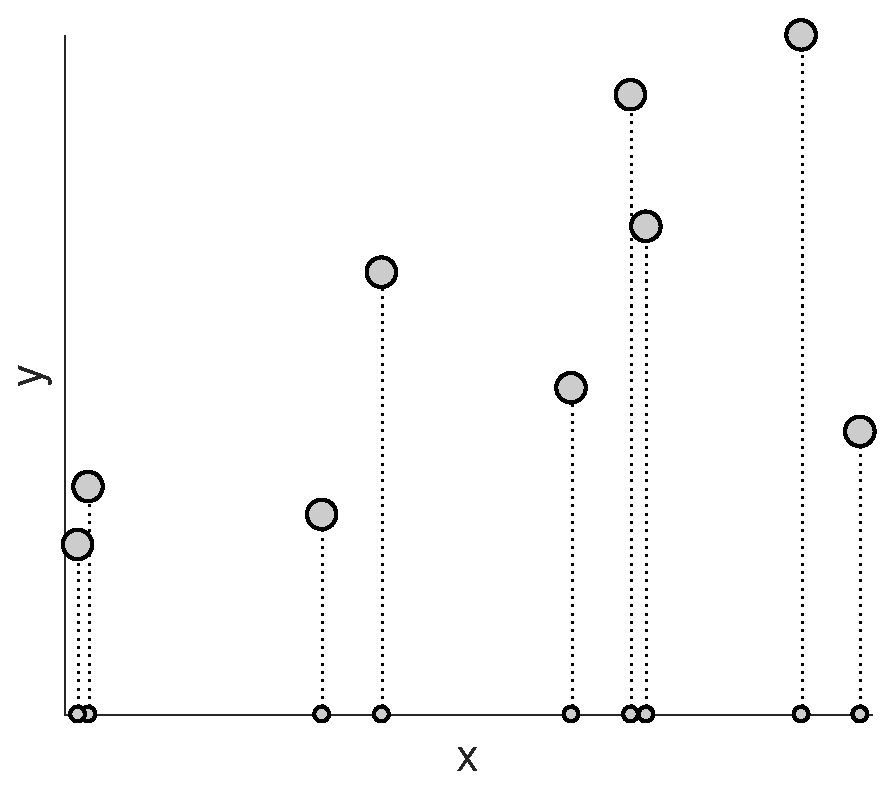
\includegraphics[width=\textwidth]{figs/regression-points}}}
\only<2->{
\centerline{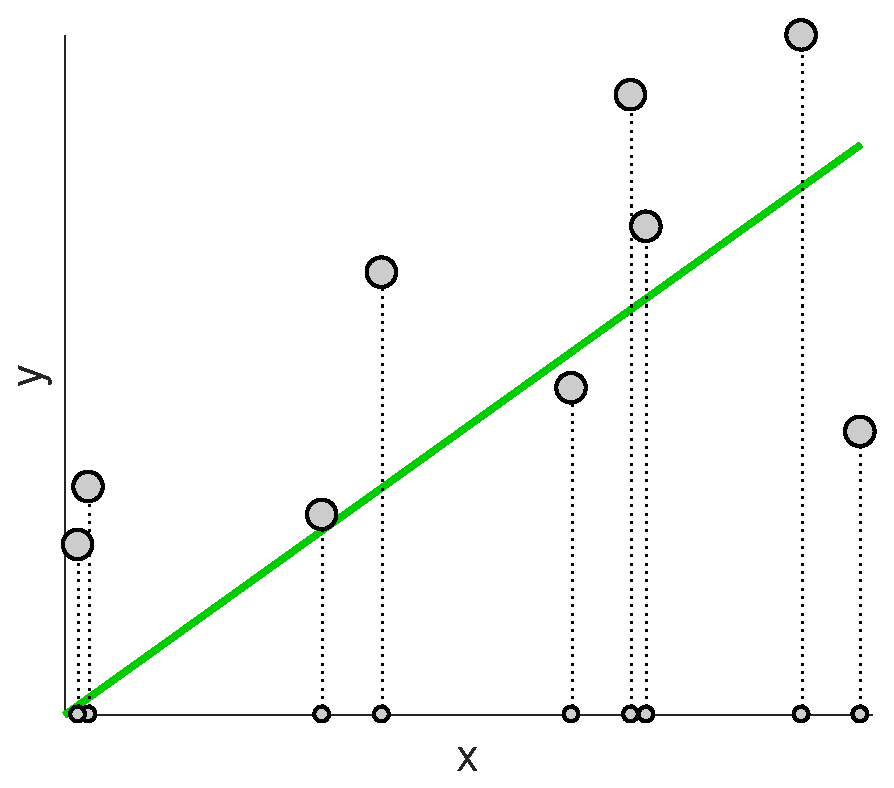
\includegraphics[width=\textwidth]{figs/regression-simple}}
\vspace{0mm}}
\end{column}
\begin{column}{0.43\textwidth}
\begin{align*}
S=(x_1,y_1),\dots,(x_n,y_n) \overset{\text{\fontsize{6}{6}\selectfont i.i.d.}}{\sim} \dxy
\end{align*}
%\vspace{1mm}
\only<1>{
\vspace{2cm}
}

\pause
\only<2-4>{
\Blue{\textbf{Statistical regression}}
\vspace{-2mm}
\begin{align*}
y &= x\!\cdot\! \Green{w^*} + \xi,\quad\E[\,\xi\,] = 0
\end{align*}
}
\only<5-6>{
\Red{\textbf{Worst-case regression}}
\vspace{-2mm}
\begin{align*}
\Green{w^*} \!= \argmin_w\, \E_\dxy\!\big[ (x\!\cdot\! w - y)^2\big]
\end{align*}
\vspace{0mm}
}
\vspace{5mm}
\end{column}
\end{columns}
\pause
Least squares estimator (Legendre, Gauss, ca.~1805)
\vspace{-2mm}
\begin{align*}
\onslide<3->{&\of{w^*}S = \argmin_w  \sum_i (x_i\!\cdot\! w - y_i)^2}\\
\onslide<4,6>{~&
\only<4>{\text{\Blue{Unbiased!}}\quad \E\big[\of{w^*}S\big] = \Green{w^*}}
\only<6>{\text{\Red{Biased!}}\quad \E\big[\of{w^*}S\big] \neq \Green{w^*}}}
\end{align*}
\vspace{-2cm}
\end{frame}

\begin{frame}
\frametitle{Correcting the worst-case bias}
\transfade<2-4>[duration=0.25]
\begin{columns}
\begin{column}{0.45\textwidth}
\centerline{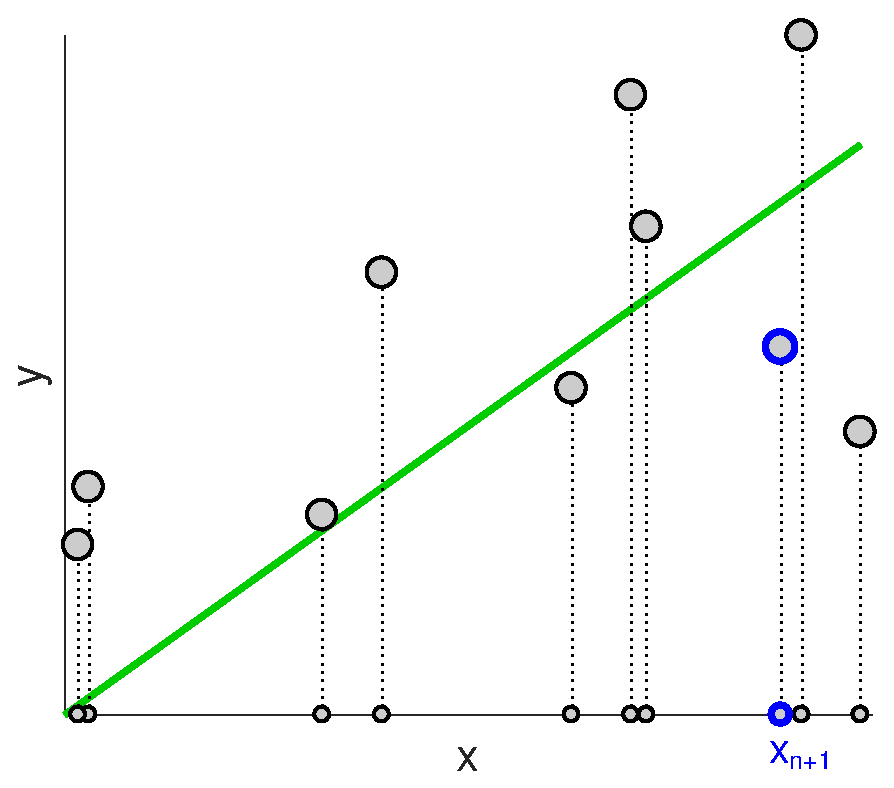
\includegraphics[width=\textwidth]{figs/regression-correction}}
\vspace{1mm}
\end{column}
\begin{column}{0.43\textwidth}
\begin{align*}
S=(x_1,y_1),\dots,(x_n,y_n) \overset{\text{\fontsize{6}{6}\selectfont i.i.d.}}{\sim} \dxy
\end{align*}
\vspace{0mm}

\Red{\textbf{Worst-case regression}}
\vspace{-5.5mm}
\begin{center}\fcolorbox{reddishyellow}{lightyellow}{
 \parbox{0.95\textwidth}{
\vspace{-5mm}
\begin{align*}
&\text{Sample}&\quad \Blue{x_{n+1}} \ &\sim\  x^2\cdot \dx\\
\onslide<2->{&\text{Query}&\quad \Blue{y_{n+1}}\ &\sim\ \dxy_{{\cal Y} |x=x_{n+1}}}
\end{align*}
\vspace{-7mm}
}}\end{center}
\pause
\vspace{2mm}
\end{column}
\end{columns}
\pause
\vspace{-2mm}
\begin{align*}
&S'\ \leftarrow\ S \ \cup\  (\Blue{x_{n+1}},\Blue{y_{n+1}})\\[2mm]
\onslide<4->{&\text{\Blue{Unbiased!}}\quad \E\big[\of{w^*}{S'}\big] = \Green{w^*}}
\end{align*}
\vspace{-2cm}
\end{frame}

\begin{frame}
\frametitle{In general: \textit{add dimension many points} \cite{correcting-bias-journal}}
\transfade<2,4->[duration=0.25]
\Red{\textbf{Worst-case regression}} in $d$ dimensions
\vspace{-1mm}
\begin{align*}
S=(\x_1,y_1),\dots,(\x_n,y_n) \overset{\text{\fontsize{6}{6}\selectfont i.i.d.}}{\sim} \dxy,
\quad\quad (\x,y)\in\R^d\!\times\! \R
\end{align*}
\pause
\Green{\textbf{Estimate the optimum}}
\vspace{-2mm}
\begin{align*}
\Green{\w^*} \!= \argmin_{\w\in\R^d}\, \E_\dxy\!\big[ (\x^\top\w - y)^2\big]
\end{align*}
\pause
\vspace{-4mm}
\begin{center}\fcolorbox{reddishyellow}{lightyellow}{
    \parbox{0.95\textwidth}{
\textit{Volume-rescaled sampling}\pause
\vspace{-4mm}
\begin{align*}
&\text{Sample}& &\Blue{\overset{\text{$d$ points}}{\x_{n+1},\dots,\x_{n+d}}}\ \sim\ \det\!
\text{\fontsize{9}{9}\selectfont$\begin{pmatrix}
-\x_{n+1}^\top-\\
\dots\\
-\x_{n+d}^\top-
\end{pmatrix}^{\!\!\!2}$} \cdot (\dx)^d\\
\onslide<5->{&\text{Query}&&\Blue{y_{n+i}}\ \sim\ \dxy_{{\cal Y} |\x=\x_{n+i}}\quad \forall_{i=1..d} }
\\[2mm]
\onslide<6->{
&\text{Add}&&\Blue{S_{\circ}} =\,  (\x_{n+1},y_{n+1}),\dots,(\x_{n+d},y_{n+d})\ \,\text{ to }\, S}
\end{align*}
\vspace{-6mm}
}}\end{center}
\pause\pause\pause
\begin{align*}
\fcolorbox{reddishyellow}{lightyellow}{\textbf{\ Theorem} \quad 
$\E\big[\of{\w^*}{S\cup \Blue{S_\circ}}\big] = \Green{\w^*}$\ }
\qquad\text{\fontsize{9}{9}\selectfont even though\quad
$\E\big[\w^*\!(S)\big] \neq \Green{\w^*}$}
\end{align*}
\end{frame}

\begin{frame}
  \frametitle{Example: averaging independent estimators}
Let $\wbh = \frac1T\sum_{t=1}^T\w^*(S_t)$, for
  independent samples $S_1,...,S_T$\pause\\[1mm]
%Error: $\|\wbh-\w^*\|$\pause\\[1mm]
\textbf{Question:} Is the estimation error $\|\wbh-\w^*\|$ converging
to 0?\pause
\begin{align*}
\text{Example:}\quad \x^\top\! = (x_1,\dots,x_5)\overset{\text{i.i.d.}}{\sim} \Nc(0,1) ,\quad\ y =
    \underbrace{\sum_{i=1}^5 x_i + \frac{x_i^3}{3}}_{\text{nonlinearity}} +\epsilon,
\end{align*}
  \centering
  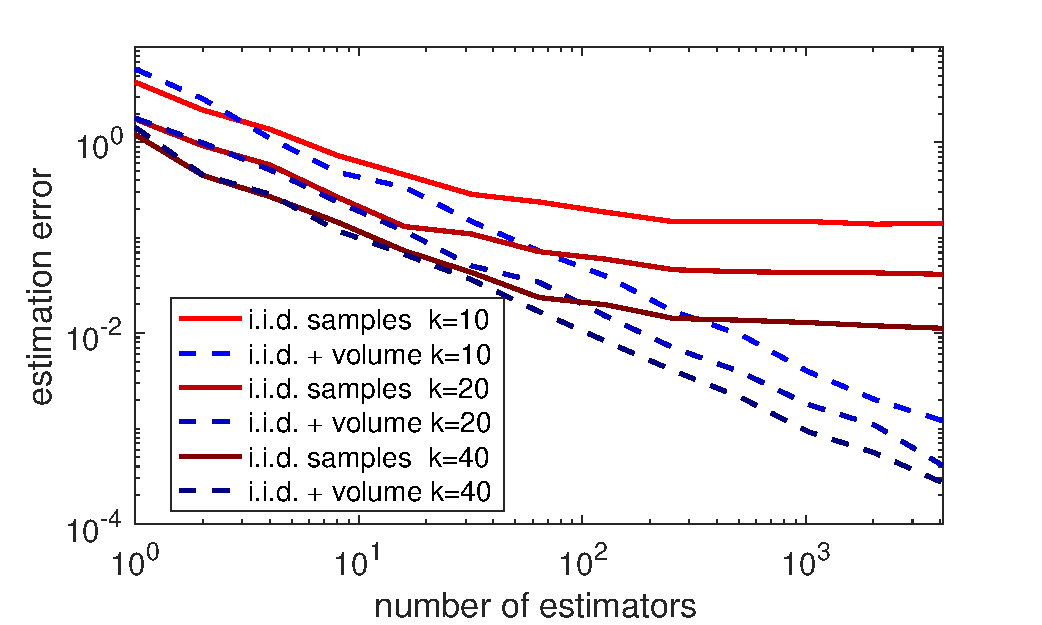
\includegraphics[width=0.7\textwidth]{../figs/gaussian}
\end{frame}

\begin{frame}
  \frametitle{Volume (determinant) as a measure of diversity}
  $\det\!
\text{\fontsize{9}{9}\selectfont$\begin{pmatrix}
-\x_{1}^\top-\\
\dots\\
-\x_{d}^\top-
\end{pmatrix}^{\!\!\!2}$}= 
\mathrm{Vol}^2\big(\{\x_1,...,\x_d\}\big)$
\pause

  \centering
  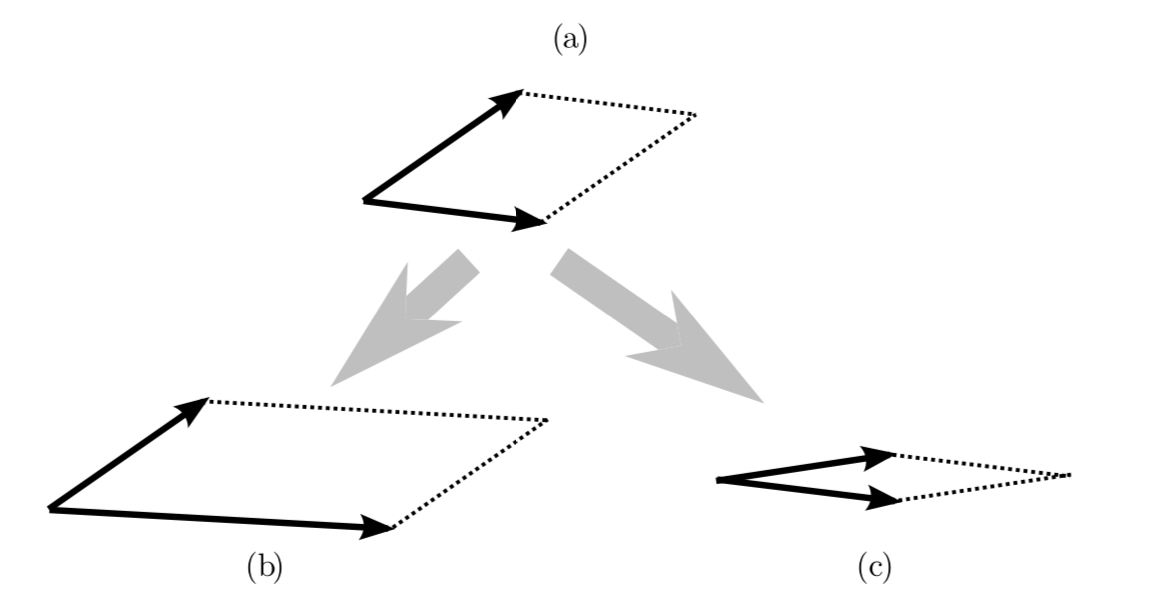
\includegraphics[width=\textwidth]{../figs/volume_illustration.png}
    \let\thefootnote\relax\footnotetext{Image from [KT12]}
\end{frame}


\begin{frame}
  \frametitle{Determinantal point processes (DPP)}
  First introduced as ``fermion processes'' by \cite{dpp-physics}\\[2mm]\pause
  \begin{quote}
No two fermions can occupy the same quantum state\quad
    \textnormal{\small (Pauli exclusion principle)}
  \end{quote}

  \begin{columns}
\begin{column}{0.5\textwidth}
     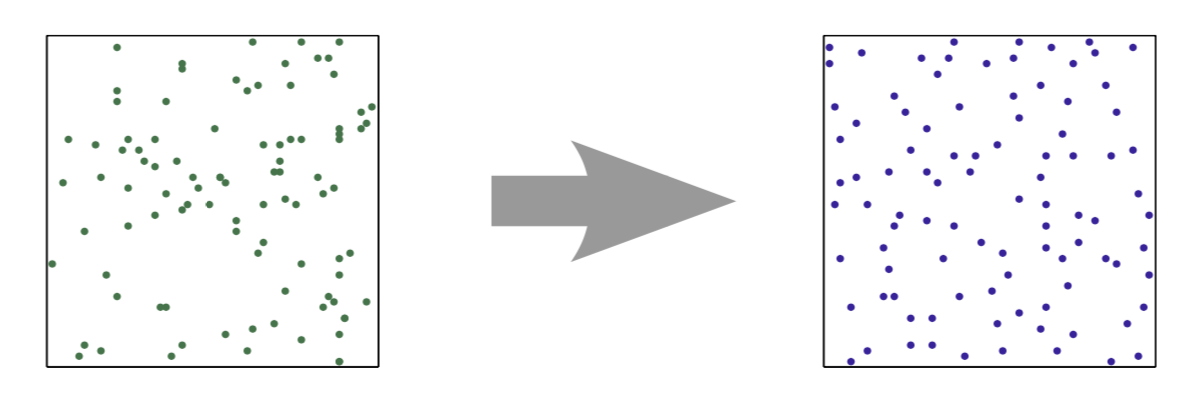
\includegraphics[width=\textwidth]{../figs/gue.png}
\end{column}
    \begin{column}{0.5\textwidth}
\pause  DPPs also appear in:\pause
  \begin{itemize}
%  \item Physics,\pause
  \item Random matrix theory \pause
  \item Graph theory \pause
  \item Optimization theory\pause
  \item Numerical linear algebra \pause
  \item Machine learning
  \end{itemize}
\end{column}
\end{columns}
\let\thefootnote\relax\footnotetext{Image from [KT12]}
\end{frame}

\begin{frame}
  \frametitle{Volume-rescaled sampling (DPP) algorithms}
  How expensive is volume-rescaled sampling?\pause
  \begin{itemize}
  \item $\dx$ is a multivariate Gaussian: $\dx=\Nc(\zero,\Sigmab)$\hfill ($\Sigmab$ unknown)\\\pause
    \textbf{Answer:} \textit{We need $2d+2$ i.i.d.~samples from $\dx$}\hfill \cite{correcting-bias}
    \pause\vspace{5mm}
  \item $\dx$ is a uniform distribution over a set $\{\x_1,...,\x_N\}$\\\pause
    \textbf{Answer:} \textit{Near-linear time sampling
      algorithm}\hfill \cite{leveraged-volume-sampling}\pause
    \vspace{5mm}
  \item $\dx$ is an arbitrary distribution with bounded support\\\pause
    \textbf{Answer:} \textit{We need $O(Kd\log d)$ i.i.d.~samples}\hfill \cite{correcting-bias-journal}
    \begin{align*}
      \text{where}\quad
      K = \sup_{\x\in\mathrm{supp}(\dx)}\x^\top\Sigmab^{-1}\x,\qquad \Sigmab=\E_{\dx}[\x\x^\top]. 
    \end{align*}
  \end{itemize}
\end{frame}


\begin{frame}
  \frametitle{Discussion}

  \begin{itemize}
  \item First-of-a-kind \emph{unbiased estimator} for worst-case regression\\[4mm]
    \pause
  \item Augmentation uses a determinantal point process (DPP) we call \emph{volume-rescaled sampling}\\[4mm]
    \pause
  \item There are many \emph{efficient DPP algorithms} \\[4mm]
    \pause
  \item A new \emph{mathematical framework} for computing expectations
\pause
  \item \emph{New applications:} \\[1mm]
    {\small  experimental design, \\
      distributed computing,\\
      stochastic optimization, ...}
  \end{itemize}
\end{frame}



\section{Volume-rescaled sampling}

\begin{frame}
\frametitle{Volume-rescaled sampling}
\begin{columns}
\begin{column}{0.6\textwidth}
\begin{align*}
\x_1,\x_2,\dots,\x_k \quad
-\quad&\text{i.i.d. random vectors}\\[-2mm]
&\text{sampled from $\x\sim\dx$}\\
\dxk\quad-\quad&
                 \text{distribution of $\X$}
  %\\[-2mm]
%&\text{random matrix $\X$}
\end{align*}
\end{column}
\begin{column}{0.3\textwidth}
\begin{center}
	\begin{tikzpicture}[scale=0.6]
          \draw [fill=brown!30] (-2,0) rectangle (0,3);
          \draw [decorate,decoration={brace}] (-2,3.1) -- (0,3.1);
          \draw (-1,3.45) node {\mbox{\fontsize{8}{8}\selectfont $d$}}; 
          \draw [color=black] (-2,2) -- (0,2);
          \draw (-2.35,2) node {\mbox{\footnotesize$\x_i^\top$}}; 
          \draw (0.2,2) node {\mbox{\fontsize{8}{8}\selectfont $i$}}; 
          \draw (0.2,2.9) node {\mbox{\fontsize{8}{8}\selectfont 1}}; 
          \draw (0.2,0.1) node {\mbox{\fontsize{8}{8}\selectfont $k$}}; 
	    \draw (-3.4,3) node {\footnotesize random $\X$}; 
	\end{tikzpicture}
\end{center}
\end{column}
\end{columns}
\vspace{4mm}
\pause

\emph{Volume-rescaled sampling} of size $k$ from $\dx$:
\begin{align*}
\vskx(\X) \propto \det(\X^\top\X)\,\dxk(\X)
\end{align*}
\pause
\textbf{Note:} For $k=d$, we have $\det(\X^\top\X)=\det(\X)^2$\pause\\[3mm]

\textbf{Question:} What is the \emph{normalization factor} of $\vskx$?
\begin{align*}
\E_{\dxk}[\det(\X^\top\X)] =\, ??
\end{align*}
\pause
We will find it through a new proof of the \emph{Cauchy-Binet formula}

\end{frame}


\begin{frame}
\frametitle{Cauchy-Binet formula}
\begin{columns}
\begin{column}{0.6\textwidth}
\begin{align*}
\x_1,\x_2,\dots,\x_n \quad
-\quad&\text{rows of matrix $\X$}
\end{align*}
\end{column}
\begin{column}{0.35\textwidth}
\begin{center}
	\begin{tikzpicture}[scale=0.6]
          \draw [fill=brown!30] (-2,0) rectangle (0,3);
          \draw [decorate,decoration={brace}] (-2,3.1) -- (0,3.1);
          \draw (-1,3.45) node {\mbox{\fontsize{8}{8}\selectfont $d$}}; 
          \draw [color=black] (-2,2) -- (0,2);
          \draw (-2.35,2) node {\mbox{\footnotesize$\x_i^\top$}}; 
          \draw (0.2,2) node {\mbox{\fontsize{8}{8}\selectfont $i$}}; 
          \draw (0.2,2.9) node {\mbox{\fontsize{8}{8}\selectfont 1}}; 
          \draw (0.2,0.1) node {\mbox{\fontsize{8}{8}\selectfont $n$}}; 
	    \draw (-3.3,3) node {\footnotesize fixed $\X$}; 
	\end{tikzpicture}
\end{center}
\end{column}
\end{columns}
\vspace{2mm}
\pause

\begin{theorem}[Cauchy-Binet]
\vspace{-6mm}
\begin{align*}
\det\!\big(\X^\top\X\big) = \sum_{S:\,|S|=d}\det\!\big(\X_S^\top\X_S\big)
\end{align*}
\vspace{-3mm}
\end{theorem}
\pause
\vspace{2mm}

Note: 
\begin{align*}
\X_S^\top\X_S = \sum_{i\in S}\x_i\x_i^\top\quad\text{is a $d\!\times\!d$ matrix},\quad S\subseteq \{1..n\}
\end{align*}
\end{frame}

\begin{frame}
\frametitle{Proof of Cauchy-Binet: Preliminaries}
Sylvester's Theorem:
\vspace{-3mm}
\begin{align*}
\det(\X^\top\X - \x_i\x_i^\top) = \det(\X^\top\X)\big(1 - \overbrace{\x_i^\top(\X^\top\X)^{+}\x_i}^{\text{$i$-th leverage score}}\big)
\end{align*}
\vspace{4mm}
\pause

Leverage score sum:
\begin{align*}
\sum_{i=1}^n \x_i^\top(\X^\top\X)^{+}\x_i = \tr(\X(\X^\top\X)^{+}\X^\top) = \rank(\X).
\end{align*}
\end{frame}

\begin{frame}
\frametitle{\only<1-8>{Proof of Cauchy-Binet}\only<9>{General proof method: $d$-modularity}}
\begin{columns}
\begin{column}{0.6\textwidth}
\begin{align*}
\only<1-7>{\x_{\sigma_1},\x_{\sigma_2},\dots,\x_{\sigma_n}\!}
\only<8->{\x_1,\x_2,\dots,\x_n} \quad
-\quad&\only<1-7>{\text{random permutation}}
\only<8->{\text{\Blue{\emph{exchangeable} sequence}}}\\
&\only<1-7>{\text{of the rows of $\X$}}\only<8->{\text{\Blue{of random vectors}}}
\end{align*}
\end{column}
\begin{column}{0.35\textwidth}
\begin{center}
	\begin{tikzpicture}[scale=0.6]
          \draw [fill=brown!30] (-2,0) rectangle (0,3);
          \draw [decorate,decoration={brace}] (-2,3.1) -- (0,3.1);
          \draw (-1,3.45) node {\mbox{\fontsize{8}{8}\selectfont $d$}}; 
          \draw [color=black] (-2,2) -- (0,2);
          \draw (-2.35,2) node {\mbox{\footnotesize \only<1-7>{$\x_{\sigma_i}^\top$}\only<8->{$\x_i^\top$}}}; 
          \draw (0.2,2) node {\mbox{\fontsize{8}{8}\selectfont $i$}}; 
          \draw (0.2,2.9) node {\mbox{\fontsize{8}{8}\selectfont 1}}; 
          \draw (0.2,0.1) node {\mbox{\fontsize{8}{8}\selectfont $n$}}; 
	    \draw (-3.5,3) node {\only<1-7>{\footnotesize permuted
                $\X^\sigma$}\only<8->{\footnotesize random $\X\ \,$}}; 
	\end{tikzpicture}
\end{center}
\end{column}
\end{columns}
\vspace{-2mm}
\pause
\only<1-2>{
\begin{align*}
\hspace{-9mm}\E\bigg[\!
\det\!\Big(\!\overbrace{%\sum_{i=1}^d\x_{\sigma_i}\x_{\sigma_i}^\top
\x_{\sigma_1}\x_{\sigma_1}^\top\!\!+\! \text{\fontsize{8}{8}\selectfont$\dots$}\!\!+\!\x_{\sigma_d}\x_{\sigma_d}^\top}^{\X_{[d]}^{\sigma\top}\X_{[d]}^{\sigma}}\!\Big)\!\bigg]
=\E\bigg[\!\det\!\Big(\!\overbrace{%\text{\fontsize{8}{8}\selectfont$
\x_{\sigma_1}\x_{\sigma_1}^\top\!\!+\!\text{\fontsize{8}{8}\selectfont$\dots
\cancel{\x_{\sigma_i}\x_{\sigma_i}^\top}\dots $}\!\!+\!\x_{\sigma_{d+1}}\x_{\sigma_{d+1}}^\top }^{\X_{[d+1]}^{\sigma\top}\X_{[d+1]}^{\sigma}-\x_{\sigma_i}\x_{\sigma_i}^\top}\!\Big)\!\bigg]
\white{\sum_{i=1}^{d+1}}\\
&\white{=\frac{1}{d\!+\!1}\sum_{i=1}^{d+1} }\\
&\white{=\frac{1}{d\!+\!1}\sum_{i=1}^{d+1} }\\
&\white{=\frac{1}{d\!+\!1}\sum_{i=1}^{d+1} }
\end{align*}
}
\only<3-7>{
\begin{align*}
\hspace{-9mm}
\E\Big[\!\det\!\big(\X_{[d]}^{\sigma\top}\X_{[d]}^{\sigma}\big)\Big]
%}^{\frac{1}{{n\choose d}}\sum_{S:|S|=d}\det(\X_S^\top\X_S)}
\ &=\quad\,
\text{\fontsize{8}{8}\selectfont$\frac{1}{d\!\!+\!\!1}$}\!\sum_{i=1}^{d+1}
\E\bigg[\!\det\!\Big(\!\overbrace{%\text{\fontsize{8}{8}\selectfont$
\x_{\sigma_1}\x_{\sigma_1}^\top\!\!+\!\text{\fontsize{8}{8}\selectfont$\dots
\cancel{\x_{\sigma_i}\x_{\sigma_i}^\top}\dots $}\!\!+\!\x_{\sigma_{d+1}}\x_{\sigma_{d+1}}^\top }^{\X_{[d+1]}^{\sigma\top}\X_{[d+1]}^{\sigma}-\x_{\sigma_i}\x_{\sigma_i}^\top}\!\Big)\!\bigg]\\
\onslide<4->{
\hspace{-9mm}\text{\fontsize{8}{8}\selectfont(Sylvester's Theorem)}\ 
&=\E\bigg[\text{\fontsize{8}{8}\selectfont$\frac{1}{d\!\!+\!\!1}$}\!
\sum_{i=1}^{d+1} 
\det\!\big(\X_{[d\!+\!1]}^{\sigma\top}\X_{[d\!+\!1]}^{\sigma}\big)\Red{\Big(1 - \x_{\sigma_i}^\top\!\big(\X_{[d\!+\!1]}^{\sigma\top}\X_{[d\!+\!1]}^{\sigma}\big)^{\!+}
\!\x_{\sigma_i}\!\Big)}\!\bigg]\\}
\onslide<5->{
\hspace{-9mm}\text{\fontsize{8}{8}\selectfont(\Red{Leverage score sum})}\ &=
\text{\fontsize{8}{8}\selectfont$\frac{\Red{(d\!+\!1) - d}}{d\!+\!1}$} \,\E\Big[\!\det\!\big(\X_{[d\!+\!1]}^{\sigma\top}\X_{[d\!+\!1]}^{\sigma}\big) \Big]\\[-3mm]}
\onslide<6->{
\dots\quad &=\Bigg[\prod_{s=d+1}^k \!\!\text{\fontsize{8}{8}\selectfont$\frac{s-d}{s}$}\Bigg]
\,\E\Big[\!\det\!\big(\X_{[k]}^{\sigma\top}\X_{[k]}^{\sigma}\big) \Big]}
\onslide<7->{\, \overset{\text{\fontsize{6}{6}\selectfont$k\!=\!n$}}{=} \text{\fontsize{8}{8}\selectfont$\frac{1}{{n\choose d}}$} \overbrace{\E\Big[\!\det\!\big(\X^{\sigma\top}\X^{\sigma}\big)\Big]}^{\det(\X^\top\X)}}
\end{align*}
}
\only<8>{
\begin{align*}
\hspace{-9mm}\E\Big[\!
\det\!\big(\X_{[d]}^{\top}\X_{[d]}\big)\Big]
\ &=\quad\,
\text{\fontsize{8}{8}\selectfont$\frac{1}{d\!\!+\!\!1}$}\!\sum_{i=1}^{d+1}
\E\bigg[\!\det\!\Big(\!\overbrace{%\text{\fontsize{8}{8}\selectfont$
\x_{1}\x_{1}^\top\!\!+\!\text{\fontsize{8}{8}\selectfont$\dots
\cancel{\x_{i}\x_{i}^\top}\dots $}\!\!+\!\x_{{d+1}}\x_{{d+1}}^\top }^{\X_{[d+1]}^{\top}\X_{[d+1]}-\x_{i}\x_{i}^\top}\!\Big)\!\bigg]\\
\hspace{-9mm}\text{\fontsize{8}{8}\selectfont(Sylvester's Theorem)}\ 
&=\E\bigg[\text{\fontsize{8}{8}\selectfont$\frac{1}{d\!\!+\!\!1}$}\!
\sum_{i=1}^{d+1} 
\det\!\big(\X_{[d\!+\!1]}^{\top}\X_{[d\!+\!1]}\big)\Red{\Big(1 - \x_{i}^\top\big(\X_{[d\!+\!1]}^{\top}\X_{[d\!+\!1]}\big)^{\!+}
\x_{i}\Big)}\bigg]\\
\hspace{-9mm}\text{\fontsize{8}{8}\selectfont(\Red{Leverage score sum})}\ &=
\text{\fontsize{8}{8}\selectfont$\frac{\Red{(d\!+\!1) - d}}{d\!+\!1}$} \,\E\Big[\!\det\!\big(\X_{[d\!+\!1]}^{\top}\X_{[d\!+\!1]}\big) \Big]\\[0.7mm]
\dots\quad &=\Bigg[\prod_{s=d+1}^k \!\!\text{\fontsize{8}{8}\selectfont$\frac{s-d}{s}$}\Bigg]
\,\E\Big[\!\det\!\big(\X_{[k]}^{\top}\X_{[k]}\big) \Big]
\, \overset{\text{\fontsize{6}{6}\selectfont$k\!=\!n$}}{=} \text{\fontsize{8}{8}\selectfont$\frac{1}{{n\choose d}}$} \,\E\Big[\!\det\!\big(\X^{\top}\X\big)\Big] %}^{\white{\det(\X^\top\X)}}
\end{align*}
}
\only<9>{
\vspace{3.25mm}
\begin{align*}
\hspace{-3.25mm}\E\Big[
F\big(\X_{[k]}\big)\Big]
\quad\, &=\quad\,
\text{\fontsize{8}{8}\selectfont$\frac{1}{k\!\!+\!\!1}$}\!\sum_{i=1}^{k+1}
\E\Big[F\big(\X_{[k\!+\!1]-i}\big)\Big]\\
&=\quad\,
\E\bigg[\text{\fontsize{8}{8}\selectfont$\frac{1}{k\!\!+\!\!1}$} \Red{\sum_{i=1}^{k+1}
F\big(\X_{[k\!+\!1]-i}\big)}\bigg]\\
% \E\bigg[\text{\fontsize{8}{8}\selectfont$\frac{1}{d\!\!+\!\!1}$}\!
% \sum_{i=1}^{d+1} 
% \det\!\big(\X_{[d\!+\!1]}^{\top}\X_{[d\!+\!1]}\big)\Big(1 - \x_{i}^\top\big(\X_{[d\!+\!1]}^{\top}\X_{[d\!+\!1]}\big)^{\!-1}
% \x_{i}\Big)\bigg]
 \hspace{-3.25mm}\text{\fontsize{8}{8}\selectfont(\Red{$d$-modularity})}\quad
        &=
\text{\fontsize{8}{8}\selectfont$\frac{\Red{(k\!+\!1) - d}}{k\!+\!1}$} \,\E\Big[
\Red{F\big(\X_{[k\!+\!1]}\big)} \Big]\\[1.1mm]
\dots\quad &=\Bigg[\prod_{s=k+1}^n \!\!\text{\fontsize{8}{8}\selectfont$\frac{s-d}{s}$}\Bigg]
\,\E\Big[F\big(\X_{[n]}\big) \Big]
% \, \overset{\text{\fontsize{6}{6}\selectfont$k\!=\!n$}}{=} \text{\fontsize{8}{8}\selectfont$\frac{1}{{n\choose d}}$} 
% \,\E\Big[F\big(\X\big)\Big]
\hspace{4.05cm}~ %}^{\white{\det(\X^\top\X)}}
\end{align*}
}
\end{frame}

\begin{frame}
  \frametitle{Application: Normalization of $\vskx$}
  \vspace{-5mm}
\begin{columns}
\begin{column}{0.6\textwidth}
\begin{align*}
\x_1,\x_2,\dots,\x_k \quad
-\quad&\text{i.i.d. random vectors}\\[-2mm]
&\text{sampled from $\x\sim\dx$}\\
\dxk\quad-\quad&
                 \text{distribution of $\X=\X_{[k]}$}
  %\\[-2mm]
%&\text{random matrix $\X$}
\end{align*}
\end{column}
\begin{column}{0.3\textwidth}
\begin{center}
	\begin{tikzpicture}[scale=0.6]
          \draw [fill=brown!30] (-2,0) rectangle (0,3);
          \draw [decorate,decoration={brace}] (-2,3.1) -- (0,3.1);
          \draw (-1,3.45) node {\mbox{\fontsize{8}{8}\selectfont $d$}}; 
          \draw [color=black] (-2,2) -- (0,2);
          \draw (-2.35,2) node {\mbox{\footnotesize$\x_i^\top$}}; 
          \draw (0.2,2) node {\mbox{\fontsize{8}{8}\selectfont $i$}}; 
          \draw (0.2,2.9) node {\mbox{\fontsize{8}{8}\selectfont 1}}; 
          \draw (0.2,0.1) node {\mbox{\fontsize{8}{8}\selectfont $k$}}; 
	    \draw (-3.3,3) node {\footnotesize random $\X$}; 
	\end{tikzpicture}
\end{center}
\end{column}
\end{columns}
\vspace{2mm}\pause
Normalization constant for volume-rescaled sampling:
\begin{align*}
\hspace{-5mm}\E_{\dxk}\!\big[\det(\X_{[k]}^\top\X_{[k]})\big] &=\lim_{n\rightarrow\infty}\bigg[\prod_{t=k+1}^n\frac{t-d}{t}\bigg]
\E\big[\det(\X_{[n]}^\top\X_{[n]})\big]\\
\onslide<3->{&=\lim_{n\rightarrow\infty}\bigg[\prod_{t=k+1}^n\frac{t\!-\!d}{t}\bigg]n^d
  \lim_{n\rightarrow\infty}\E\bigg[\det\Big(\frac1n\X_{[n]}^\top\X_{[n]}\Big)\bigg]}\\
\onslide<4->{&\overset{(*)}{=}  \underbrace{\bigg[\!\lim_{n\rightarrow\infty}\prod_{t=0}^{d-1}
  \frac{n}{n\!-\!t}\bigg]}_{1}
  \underbrace{k\,(k\!-\!1)\dots(k\!-\!d\!+\!1)}_{d!{k\choose d}} \det\!\big(\E[\x\x^\top]\big)}
\end{align*}
\vspace{0mm}

\only<4->{\let\thefootnote\relax  \footnotetext{ $(*)$ \ Law of large numbers (details omitted)}}
\end{frame}

\begin{frame}
  \frametitle{Application: Inverse expectations for $\vskx$}
Let $\X^\dagger=(\X^\top\X)^{-1}\X^\top$ denote the Moore-Penrose pseudoinverse,\\
\pause
i.e. the unique matrix such that for all vectors $\y$,\vspace{-3mm}
\begin{align*}
  \argmin_{\w}\|\X\w-\y\|^2 = \X^\dagger\y.
\end{align*}\pause
For $\X\sim\dxk$ and $\Xt\sim\vskx$, we have
  \begin{align*}
    \E[\Xt^\dagger] &= \big(\E[\X^\top\X]\big)^{-1}\E[\X]^\top
    \\[6mm]
\onslide<4->{\E\big[\Xt^\dagger\Xt^{\dagger\top}\big] &\overset{(*)}{=} \frac k{k-d+1}\cdot \big(\E[\X^\top\X]\big)^{-1}}
  \end{align*}
  \pause 
  \only<4->{
    \let\thefootnote\relax  \footnotetext{ If $\rank(\X)<d$ with probability $>0$ then $(*)$ becomes a psd inequality $\preceq$. }}
  \pause
  
\small Also leads to unbiasedness of least squares for volume-rescaled sampling

\end{frame}


\begin{frame}
  \frametitle{The decomposition of volume-rescaled sampling}
Let $\Xt\sim\vskx$ and $S\subseteq[k]$ be a random size $d$ set
such that
\begin{align*}
  \Pr(S\,|\,\Xt)\propto \det(\Xt_S)^2.
\end{align*}
\pause
\begin{columns}
  \begin{column}{0.5\textwidth}
  Then:
  \begin{itemize}
  \item $\Xt_S\sim\vsdx$,
  \item $\Xt_{[k]\backslash S}\sim \dx^{k-d}$,
  \item $S$ is uniformly random,
  \end{itemize}
  \vspace{3mm}
  
  and the three are independent.
\end{column}
\begin{column}{0.4\textwidth}
\begin{tikzpicture}[scale=0.8]
    \draw (0,0) rectangle (2,4);
    \draw[fill=blue!30] (0,1.3) rectangle (2,3.5);
    \draw (1,2.55) node {\mbox{\footnotesize $\Blue{\Xt_S}$}};
    \draw [decorate,decoration={brace}] (-.1,1.3) -- (-.1,3.5);
    \draw (-.5,2.45) node {\mbox{\fontsize{8}{8}\selectfont $d$}};
    \draw (-1.3,4) node {\footnotesize random $\Xt$}; 
  \end{tikzpicture}
\end{column}
\end{columns}
\end{frame}

\begin{frame}
  \frametitle{Consequences for least squares}
\begin{theorem}[\cite{correcting-bias}]\label{t:augmenting}
  Let $S \!=\! \{(\x_1,y_1),\textnormal{\fontsize{6}{6}\selectfont \dots},(\x_k,y_k)\}
  \overset{\textnormal{\fontsize{6}{6}\selectfont i.i.d.}}{\sim}
  D^k$, for any $k\geq 0$.\pause
\begin{align*}
&\textnormal{Sample}& &\xbt_{1},\dots,\xbt_{d}\ \sim\ \vsdx,\\
    &\textnormal{Query}&&\yt_{i}\ \sim\ D_{{\cal Y} |\x=\xbt_{i}}\quad \forall_{i=1..d}.
\end{align*}
\pause
Then for $S_{\circ}=\{(\xbt_{1},\yt_{1}),\dots,(\xbt_{d},\yt_{d})\}$,
\begin{align*}
 \E\big[\w^*( S\cup S_{\circ})\big] &= \E_{S\sim
  D^k}\!\big[\, \E_{S_{\circ}\sim \vsd}[\,\w^*(S\cup S_{\circ})\,]\, \big]\\[1mm]
\onslide<4->{\textnormal{(decomposition)}\quad&=\E_{\tilde S \sim \vs{k+d}}
\big[\,\w^*\!(\tilde S)\,\big] }\\
\onslide<5->{\textnormal{($d$-modularity)}\quad  &= \w^*.}
\end{align*}
\end{theorem}

\end{frame}



\section{Conclusions}

\begin{frame}
  \frametitle{Conclusions}
  \begin{itemize}
  \item New family of unbiased estimators for least squares\vspace{3mm}
  \item New method for computing expectations of matrix inverses\vspace{3mm}
  \item Applications in distributed computing, experimental design, etc.
  \end{itemize}
  
\end{frame}

\begin{frame}
\centering  \Large Thank you
\end{frame}

% \appendix

% \section{Minimax experimental design}
% \begin{frame}
%   \frametitle{Classical experimental design}
%   Consider $n$ parameterized experiments:
%   $\x_1,\dots,\x_n\in\R^d$.\\
%   Each experiment has a real random response $y_i$ such that:
%   \begin{align*}
%     y_i = \x_i^\top\w^* + \xi_i,\qquad \xi_i\sim\Nc(0,\sigma^2)
%   \end{align*}
%   \pause
% \textbf{Goal:} Select $k\ll n$ experiments to best estimate $\w^*$
%   \pause
% \begin{columns}
% \begin{column}{0.3\textwidth}
% \\ \vspace{0.8cm}
% Select $S=\{4,6,9\}$\\
% \vspace{1cm}
% Receive $y_4, y_6, y_9$
% \end{column}
% \begin{column}{0.5\textwidth}
% \begin{center}
% 	\begin{tikzpicture}[scale=0.9]
%           \draw [fill=brown!30] (-2,0) rectangle (0,3);
%           \draw [color=black] (-2,2) -- (0,2);
%           \draw (-2.25,2) node {\mbox{\footnotesize $\x_4^\top$}}; 
%           \draw [color=black] (-2,1.5) -- (0,1.5);
%           \draw (-2.25,1.5) node {\mbox{\footnotesize $\x_6^\top$}}; 
%           \draw [color=black] (-2,0.5) -- (0,0.5);
%           \draw (-2.25,0.5) node {\mbox{\footnotesize $\x_9^\top$}}; 
% 	   \draw (-3,3) node {fixed $\X$}; 
%            \draw [decorate,decoration={brace}] (-2,3.1) -- (0,3.1);
%           \draw (-1,3.4) node {\mbox{\fontsize{8}{8}\selectfont $d$}}; 
%             \draw [color=lightgray,line width =0.5mm] (1,0) -- (1,3);
%             \draw [color=lightgray] (0.75,3) node {$\y$};
%             \draw (0.75,2) node {\mbox{\footnotesize $y_4$}}; 
%             \draw (1,2) node {.}; 
%             \draw[mark=*,mark size=1.5pt] plot coordinates{(1,2)};
%             \draw (0.75,1.5) node {\mbox{\footnotesize $y_6$}}; 
%             \draw (1,1.5) node {.}; 
%             \draw[mark=*,mark size=1.5pt] plot coordinates{(1,1.5)};
%             \draw (0.75,0.5) node {\mbox{\footnotesize $y_9$}}; 
%             \draw[mark=*,mark size=1.5pt] plot coordinates{(1,.5)};
% 	\end{tikzpicture}
% \end{center}
% \end{column}
% \end{columns}

% \end{frame}

% \begin{frame}
%   \frametitle{A-optimal design}
%   Find an unbiased estimator $\wbh$ with smallest
%   \textit{mean squared error}:
%   \begin{align*}
%     \min_{\wbh}\max_{\w^*}\quad
%     \underbrace{\E_{\wbh}\big[\|\wbh-\w^*\|^2\big]}_{\mathrm{MSE}[\wbh]}\quad\text{subject
%     to}\quad\E\big[\wbh\big]=\w^*\ \ \forall_{\w^*}
%   \end{align*}
%   \pause
% Given every $y_1,\dots,y_n$, the optimum is \textit{least squares}: $\wbh=\X^\dagger\y$
%   \begin{align*}
% \MSE{\X^\dagger\y}=\tr\big(\Var[\X^\dagger\y]\big)=\sigma^2\underbrace{\tr\big((\X^\top\X)^{-1}\big)}_{\phi}
%   \end{align*}
%   \pause
%   \vspace{-4mm}
  
% \begin{center}\fcolorbox{reddishyellow}{lightyellow}{
%  \parbox{0.95\textwidth}{  
%    \textbf{Theorem} (based on \cite{avron-boutsidis13})\\
%    There is an experimental design $S$ of size
% $k\leq\Blue{d+\phi/\epsilon}$ such that
% $$\mathrm{MSE}[\X_S^\dagger\y_S]\leq \epsilon\cdot \tr(\Var[\xib])$$
% }}\end{center}
% \pause
% \Red{
%     Required assumption:\quad $y_i = \x_i^\top\w^* +
%     \xi_i,\quad\xi_i\sim\Nc(0,\sigma^2)$
%   }
% \end{frame}

% \begin{frame}
%   \frametitle{What if $\xi_i$ is not $\Nc(0,\sigma^2)$?}
%   \begin{align*}
%     \y&\text{ - any random vector in $\R^n$ with finite second moment}
%     \\
% \onslide<2->{    \w^*_{\y|\X}&\defeq  \argmin_\w \E_\y \big[\|\X\w-\y\|^2\big]
% }
%     \\ \onslide<3->{\xib_{\y|\X}&\defeq \y-\X\w^* }
%   \end{align*}
%   \pause\pause\pause\vspace{3mm}

% Two special cases:\vspace{2mm}
% \pause
% \begin{enumerate}
% \item Statistical regression:\quad\quad\  $\E\big[\xib_{\y|\X}\big]=\zero$
%   \pause
% \item Worst-case regression:\quad $\Var\big[\xib_{\y|\X}\big]=\zero$
% \end{enumerate}

% \end{frame}

%   \begin{frame}
%     \frametitle{Minimax experimental design}
%     \begin{theorem}[\cite{minimax-experimental-design}]
% For any $\epsilon>0$, there is a random experimental design $(S,\wbh)$
% of size
% \[k=O(\Blue{d}\log n\Blue{\,+\,\phi/\epsilon}), \quad\text{where}\quad\phi=\tr\big((\X^\top\X)^{-1}\big),\]
% such that for any random $\y$ we have
% \begin{align*}
% \text{(unbiasedness)}\quad  \E\big[\wbh(\y_S)\big]&= \w^*_{\y|\X},\\[3mm]
% \mathrm{MSE}\big[\wbh(\y_S)\big] - \mathrm{MSE}\big[\X^\dagger\y\big]
%   &\leq \epsilon\cdot 
%   \E\big[\|\xib_{\y|\X}\|^2\big]%\quad\text{and}\quad k= O(d\log n + \phi/\epsilon).
% \end{align*}
% \end{theorem}
% % \pause\vspace{4mm}

% % \textit{Toy example:} \quad$\Var[\xib_{\y|\X}]=\sigma^2\I$,\quad\ 
% % $\E[\xib_{\y|\X}]=\zero$
% % \pause\vspace{3mm}
% % \begin{enumerate}
% %   \item $\E\big[\|\xib_{\y|\X}\|^2\big]
% %     %\tr\big(\Var[\xib_{\y|\X}]\big) + \big\|\E[\xib_{\y|\X}]\big\|^2
% %     =\tr\big(\Var[\xib_{\y|\X}]\big)$
% %     \pause\vspace{1mm}
% %   \item $\MSE{\X^\dagger\y} %= \sigma^2\phi    %\leq \sigma^2k\epsilon\ll
% %     % \sigma^2n \epsilon
% %     = \frac\phi n\cdot \tr\big(\Var[\xib_{\y|\X}]\big)$
% %   \end{enumerate}
%   % \pause\vspace{3mm}
  
%   % So in this case $\mathrm{MSE}\big[\wbh(\y_S)\big]\leq
%   % O(\epsilon) \cdot \tr\big(\Var[\xib_{\y|\X}]\big)$ as expected
% \end{frame}

% \begin{frame}
%   \frametitle{Important special instances}
%   \begin{enumerate}
%   \item    \textit{Statistical regression:}\quad
%     $\y = \X\w^*+\xib$,\quad $\E[\xib]=\zero$
%     \begin{align*}
%       \mathrm{MSE}\big[\wbh(\y_S)\big] -
%       \mathrm{MSE}\big[\X^\dagger\y\big]\leq \epsilon\cdot\tr\big(\Var[\xib]\big)
%     \end{align*}
%     \pause\vspace{-5mm}
%     \begin{itemize}
%     \item Weighted regression:\quad\ 
%       $\Var[\xib]=\mathrm{diag}\big([\sigma_1^2,\dots,\sigma_n^2]\big)$\\[2mm]
%       \pause
%       \item Generalized regression: $\Var[\xib]$ is
%         arbitrary\\[2mm]
%         \pause
%         \item Bayesian regression: \quad \,$\w^*\sim\Nc(\zero,\I)$
%         \end{itemize}
%         \pause\vspace{5mm}
%       \item \textit{Worst-case regression:}\quad $\y$ is any fixed vector in
%         $\R^n$
%         \pause
%         \begin{align*}
%       \E_{S,\wbh}\big[\|\wbh(\y_S)-\w^*\|^2\big]\leq \epsilon\cdot
%           \|\y-\X\w^*\|^2
%         \end{align*}
% where $\w^*=\X^\dagger\y$
%   \end{enumerate}
% \end{frame}


% \begin{frame}
% \frametitle{Key idea: volume-rescaled \emph{importance} sampling}
% \begin{columns}
% \begin{column}{0.57\textwidth}
%   \vspace{3mm}

%   Simple volume-rescaled sampling:
%   \begin{itemize}
%   \item Let $\dx$ be a uniformly random $\x_i$
%   \item $(\X_S,\y_S)\sim \vsk$ and $\wbh=\X_S^\dagger\y_S$.
%   \end{itemize}
%   \vspace{4mm}
  
%   Then, $\E[\wbh] = \w^*_{\y|\X}$.
% \end{column}
% \begin{column}{0.4\textwidth}
% \begin{center}
% 	\begin{tikzpicture}[scale=0.9]
%           \draw [fill=brown!30] (-2,0) rectangle (0,3);
%           \draw [color=black] (-2,2) -- (0,2);
%           \draw (-2.25,2) node {\mbox{\footnotesize $\x_4^\top$}}; 
%           \draw [color=black] (-2,1.5) -- (0,1.5);
%           \draw (-2.25,1.5) node {\mbox{\footnotesize $\x_6^\top$}}; 
%           \draw [color=black] (-2,0.5) -- (0,0.5);
%           \draw (-2.25,0.5) node {\mbox{\footnotesize $\x_9^\top$}}; 
% 	   \draw (-2.7,3) node {\footnotesize fixed $\X$}; 
%            \draw [decorate,decoration={brace}] (-2,3.1) -- (0,3.1);
%           \draw (-1,3.4) node {\mbox{\fontsize{8}{8}\selectfont $d$}}; 
%             \draw [color=lightgray,line width =0.5mm] (1,0) -- (1,3);
%             \draw [color=lightgray] (0.75,3) node {$\y$};
%             \draw (0.75,2) node {\mbox{\footnotesize $y_4$}}; 
%             \draw (1,2) node {.}; 
%             \draw[mark=*,mark size=1.5pt] plot coordinates{(1,2)};
%             \draw (0.75,1.5) node {\mbox{\footnotesize $y_6$}}; 
%             \draw (1,1.5) node {.}; 
%             \draw[mark=*,mark size=1.5pt] plot coordinates{(1,1.5)};
%             \draw (0.75,0.5) node {\mbox{\footnotesize $y_9$}}; 
%             \draw[mark=*,mark size=1.5pt] plot coordinates{(1,.5)};
% 	\end{tikzpicture}
% \end{center}
% \end{column}
% \end{columns}
% \vspace{5mm}
% \pause

% \textbf{Problem:} \ Not robust to worst-case noise\\
% \pause

% \textbf{Solution:} Volume-rescaled importance sampling\\[1mm]
% \pause
% \begin{itemize}
% \item Let $p=(p_1,\dots,p_n)$ be an importance sampling distribution,
% \item Define $\xbt\sim\dx$ as $\xbt=\frac1{\sqrt{p_i}}\x_i$ for $i\sim p$.
% \end{itemize}
% \pause
% Then, for $(\Xt_S,\ybt_S)\sim\vsk$ and $\wbh = \Xt_S^\dagger\ybt_S$,
% we have $\E[\wbh]=\w_{\y|\X}^*$.
% \end{frame}

% \begin{frame}
%   \frametitle{Importance sampling for experimental design}
%   \begin{enumerate}
%   \item  \textit{Leverage score sampling}: $\Pr(i)=p_i^{\mathrm{lev}}
% \defeq \frac1d \x_i^\top(\X^\top\X)^{-1}\x_i$\\
% {\footnotesize A standard sampling method for worst-case linear regression.}
% \pause
% \vspace{5mm}

%   \item \textit{Inverse score sampling}: $\Pr(i)= p_i^{\mathrm{inv}}\defeq
%     \frac1\phi\x_i^\top(\X^\top\X)^{-2}\x_i$.\\
% {\footnotesize  A novel sampling technique essential
%     for achieving $O(\phi/\epsilon)$ sample size.}
%   \end{enumerate}
% \end{frame}

% \begin{frame}
%   \frametitle{Minimax A-optimality}
%   \begin{definition}
%     Minimax A-optimal value for experimental design:
% \begin{align*}
% R_k^*(\X)&\defeq 
%   \min_{(S,\wbh)\in\Wc_k(\X)}\ \max_{\y\in\Fc_n\backslash\mathrm{Sp}(\X)}\,\frac{\mathrm{MSE}\big[\wbh(\y_S)\big]-
%      \mathrm{MSE}\big[\X^\dagger\y\big]
%   }{\E\big[\|\xib_{\y|\X}\|^2\big]}
% \end{align*}
% \end{definition}
% \pause
% % \textbf{Fact.} \ $\X^\dagger\y$ is the \textit{minimum
% %   variance unbiased estimator} for $\Fc_n$:
% % \begin{align*}
% %   \text{if}\quad  \E_{\y,\wbh}\big[\wbh(\y)\big]
% %   &=\X^\dagger\E[\y]\quad\quad\,\forall_{\y\in\Fc_n}
% % \\ \text{then}\quad
% %   \Var\big[\wbh(\y)\big]&\succeq\Var\big[\X^\dagger\y\big]\quad \forall_{\y\in\Fc_n}
% % \end{align*}
% \begin{itemize}
% \item If \ $d\leq k\leq n$,\qquad\quad then \
%   $R_k^*(\X)\in[0,\infty)$
%     \pause
% \item If \ $k\geq C\cdot d\log n$,\quad \,then \ $R_k^*(\X)\leq
%   C\cdot\phi/k$\hfill for some $C$
% \pause
% \item If \ $k^2<\epsilon nd/3$,\qquad\ \,then \ $R_k^*(\X)\geq
%     (1\!-\!\epsilon)\cdot\phi/k$\hfill for some $\X$
% \end{itemize}
% \end{frame}


% \section{Bayesian experimental design}

% \begin{frame}
%   \frametitle{Bayesian experimental design}
%   Consider $n$ parameterized experiments:
%   $\x_1,\dots,\x_n\in\R^d$.\\
%   Each experiment has a real random response $y_i$ such that:
%   \begin{align*}
%     y_i = \x_i^\top\w^* + \xi_i,\qquad \xi_i\sim\Nc(0,\sigma^2),\quad \Blue{\w^*\sim\Nc(\zero,\sigma^2\A^{-1})}
%   \end{align*}
%   \pause
% \textbf{Goal:} Select $k\ll n$ experiments to best estimate $\w^*$
% \begin{columns}
% \begin{column}{0.3\textwidth}
% \\ \vspace{0.8cm}
% Select $S=\{4,6,9\}$\\
% \vspace{1cm}
% Receive $y_4, y_6, y_9$
% \end{column}
% \begin{column}{0.5\textwidth}
% \begin{center}
% 	\begin{tikzpicture}[scale=0.9]
%           \draw [fill=brown!30] (-2,0) rectangle (0,3);
%           \draw [color=black] (-2,2) -- (0,2);
%           \draw (-2.25,2) node {\mbox{\footnotesize $\x_4^\top$}}; 
%           \draw [color=black] (-2,1.5) -- (0,1.5);
%           \draw (-2.25,1.5) node {\mbox{\footnotesize $\x_6^\top$}}; 
%           \draw [color=black] (-2,0.5) -- (0,0.5);
%           \draw (-2.25,0.5) node {\mbox{\footnotesize $\x_9^\top$}}; 
% 	   \draw (-2.8,3) node {\footnotesize fixed $\X$}; 
%            \draw [decorate,decoration={brace}] (-2,3.1) -- (0,3.1);
%           \draw (-1,3.4) node {\mbox{\fontsize{8}{8}\selectfont $d$}}; 
%             \draw [color=lightgray,line width =0.5mm] (1,0) -- (1,3);
%             \draw [color=lightgray] (0.75,3) node {$\y$};
%             \draw (0.75,2) node {\mbox{\footnotesize $y_4$}}; 
%             \draw (1,2) node {.}; 
%             \draw[mark=*,mark size=1.5pt] plot coordinates{(1,2)};
%             \draw (0.75,1.5) node {\mbox{\footnotesize $y_6$}}; 
%             \draw (1,1.5) node {.}; 
%             \draw[mark=*,mark size=1.5pt] plot coordinates{(1,1.5)};
%             \draw (0.75,0.5) node {\mbox{\footnotesize $y_9$}}; 
%             \draw[mark=*,mark size=1.5pt] plot coordinates{(1,.5)};
% 	\end{tikzpicture}
% \end{center}
% \end{column}
% \end{columns}
% \end{frame}

% \begin{frame}
%   \frametitle{Bayesian A-optimal design}
% Given the Bayesian assumptions, we have
%   \begin{align*}
%   \w\mid \y_S \ \sim\ \Nc\Big(\ (\X_S^\top\X_S + \A)^{-1}\X_S^\top\y_S
%   ,\ \ \sigma^2(\X_S^\top\X_S+\A)^{-1}\ \Big),
%   \end{align*}
%   \pause
  
%   Bayesian A-optimality criterion:
% \begin{align*}
% f_{\A}(\X_S^\top\X_S)=\tr\big((\X_S^\top\X_S+\A)^{-1}\big).
% \end{align*}
% \pause

% \textbf{Goal:} Efficiently find subset $S$ of size $k$ such that:
% \begin{align*}
% f_{\A}(\X_S^\top\X_S)\leq (1+\epsilon)\cdot\underbrace{\min_{S':|S'|=k}f_{\A}(\X_{S'}^\top\X_{S'})}_{\opt}
% \end{align*}
% \end{frame}

% \begin{frame}
%   \frametitle{Relaxation to a semi-definite program}
%   \begin{block}{SDP relaxation}
% The following can be found via an SDP solver in polynomial time:
%   \begin{align*}
% p^* \ = \  \argmin_{p_1,...,p_n}\ \
%   f_{\A}\Big(\sum_{i=1}^np_i\x_i\x_i^\top\Big),\\
% \text{subject to}\quad
%   \forall_i\ \ 0\leq p_i\leq 1,\quad \sum_i p_i=k.
%   \end{align*}
%   \vspace{-5mm}
% \end{block}
% \pause
% \vspace{5mm}

% The solution $p^*$ satisfies $f_{\A}\big(\sum_{i}p_i\x_i\x_i^\top\big)\leq\opt$.\\[5mm]
% \pause

% \textbf{Question:}
% For what $k$ can we efficiently round this to $S$ of size $k$?
    
% \end{frame}

% \begin{frame}
%   \frametitle{Efficient rounding for \emph{effective dimension} many
%     points}
%   \begin{definition}
% Define $\A$-effective dimension as $d_{\A} =\tr\big(\X^\top\X(\X^\top\X+\A)^{-1}\big) \leq d$.
% \end{definition}
% \pause
%   \begin{theorem}[\cite{bayesian-experimental-design}]
% If $k=\Omega\big(\frac{d_{\A}}{\epsilon} +
% \frac{\log1/\epsilon}{\epsilon^2}\big)$,
% then there is a polynomial time 
%   algorithm that finds subset $S$ of size $k$ such that
%   \begin{align*}
%     f_{\A}\big(\X_S^\top\X_S\big) \leq (1+\epsilon)\cdot\opt.
%   \end{align*}
% \end{theorem}
% \vspace{2mm}
% \pause
% \textbf{Remark:} Extends to other Bayesian criteria:
% C/D/V-optimality.\\[3mm]
% \pause
% \textbf{Key idea:} \ Rounding with \emph{$\A$-regularized}
% volume-rescaled sampling,\\
% a new kind of determinantal point process.
% \end{frame}

% \begin{frame}
%   \frametitle{Comparison with prior work}
%   \centering
%     \renewcommand{\arraystretch}{1.5}
% \begin{tabular}{r||c|c|l}
%  &Criteria&Bayesian&$k=\Omega(\cdot)$\\
%   \hline\hline
% \small \cite{tractable-experimental-design}
%   &\small A,V&\xmark&$\frac{d^2}{\epsilon}$\\
% \small \cite{near-optimal-design}
%   &\small A,C,D,E,G,V&\cmark&$\frac {d}{\epsilon^2}$\\
% \small  \cite{proportional-volume-sampling}
%   &\small A,D&\xmark&$\frac{d}{\epsilon} +
%   \frac{\log1/\epsilon}{\epsilon^2}$\\
%   \hline
% \small\textbf{our result} \cite{bayesian-experimental-design}&\small A,C,D,V&\cmark& $\frac{d_{\A}}{\epsilon} +
%   \frac{\log1/\epsilon}{\epsilon^2}$
% \end{tabular}
% \end{frame}

\begin{frame}[allowframebreaks]
  \frametitle{References}
  \scriptsize 
  \bibliographystyle{alpha}
  \bibliography{../pap}
\end{frame}


\end{document}
